\documentclass[12pt,letterpaper]{article}

\usepackage{assignments}
% \usepackage{minted}
\usepackage{graphicx}
\usepackage{subcaption}

\begin{document}

\title{\vspace{-4ex}ECE521: Inference Algorithms and Machine Learning \\
University of Toronto\\ \  \\
Solution to Assignment 3: \\Unsupervised Learning and Probabilistic Models}
\author{Renjie Liao}
% \date{\vspace{-8ex}TA: Use Piazza for Q\&A \\ Due date: Mar. 24 11:59 pm, 2017 \\ Electronic submission to: \href{mailto:ece521ta@gmail.com}{ece521ta@gmail.com} }


\maketitle

\begin{mycomments}
\section{Part 1}
\end{mycomments}
\section{K-means}

\subsection{Learning K-means [8 pt.]}

\begin{figure}
    \centering
    \begin{subfigure}[b]{0.45\textwidth}
        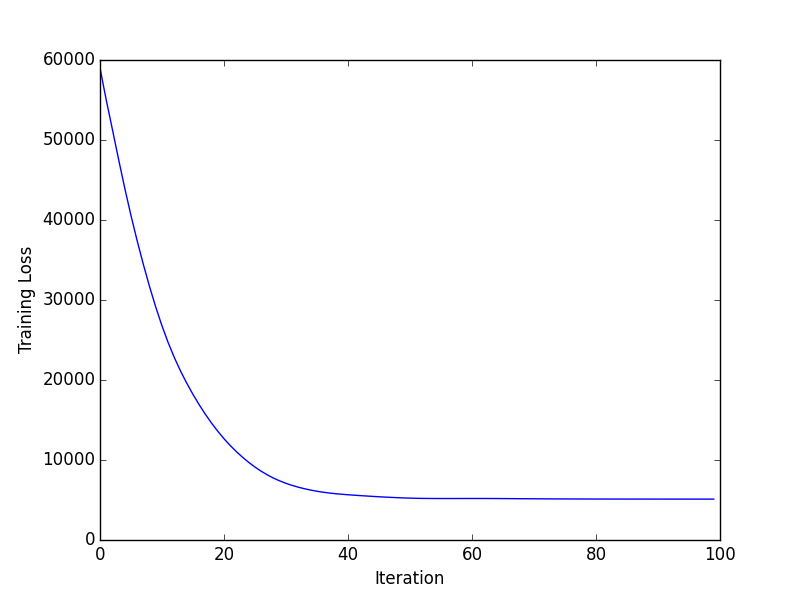
\includegraphics[width=\textwidth]{imgs/kmeans_train_loss.png}
        \caption{1.1.2, Training loss}
    \end{subfigure}
    \begin{subfigure}[b]{0.45\textwidth}
        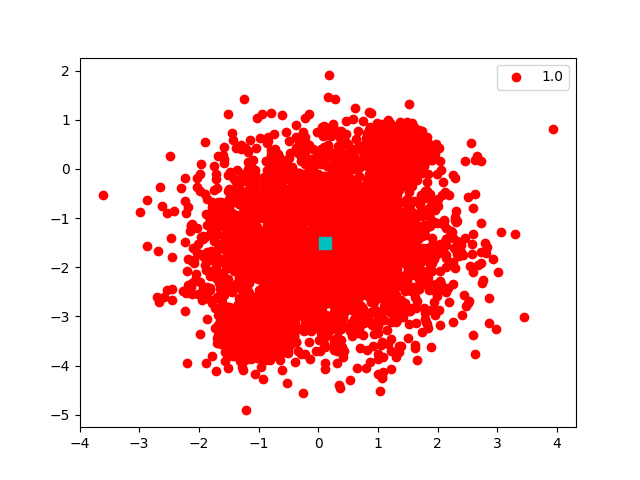
\includegraphics[width=\textwidth]{imgs/kmeans_K_1.png}
        \caption{1.1.3, K = 1}
    \end{subfigure}

    \begin{subfigure}[b]{0.45\textwidth}
        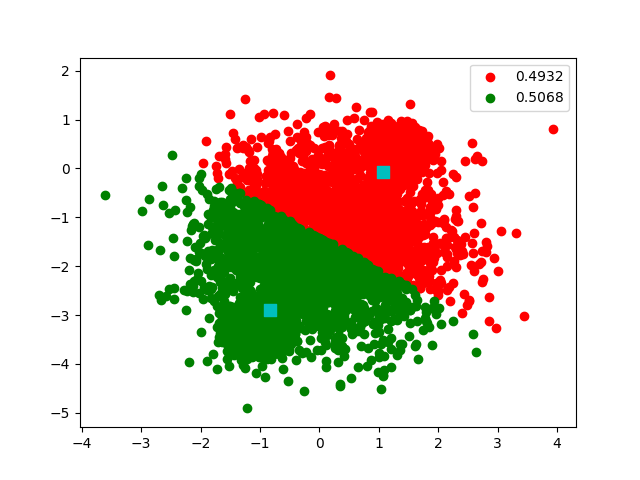
\includegraphics[width=\textwidth]{imgs/kmeans_K_2.png}
        \caption{1.1.3, K = 2}
    \end{subfigure}
    \begin{subfigure}[b]{0.45\textwidth}
        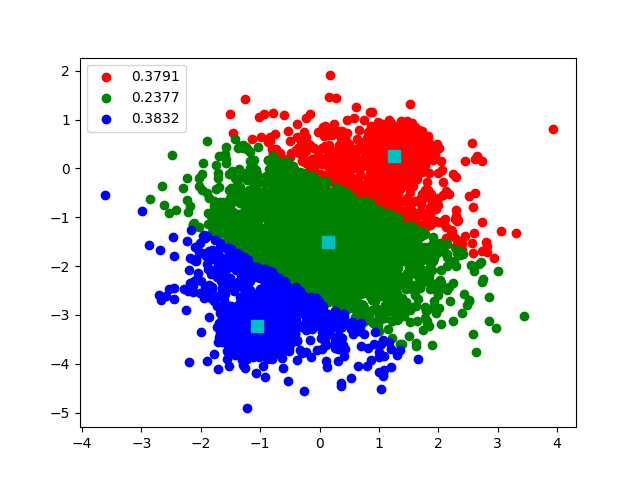
\includegraphics[width=\textwidth]{imgs/kmeans_K_3.png}
        \caption{1.1.3, K = 3}
    \end{subfigure}
     
    %add desired spacing between images, e. g. ~, \quad, \qquad, \hfill etc. 
    %(or a blank line to force the subfigure onto a new line)
    \begin{subfigure}[b]{0.45\textwidth}
        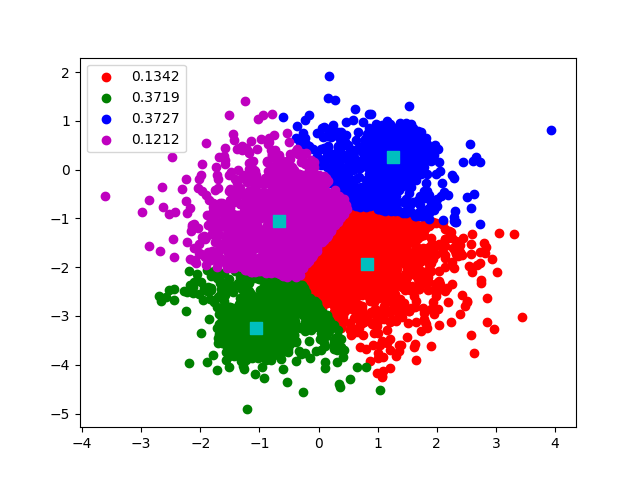
\includegraphics[width=\textwidth]{imgs/kmeans_K_4.png}
        \caption{1.1.3, K = 4}
    \end{subfigure}
    \begin{subfigure}[b]{0.45\textwidth}
        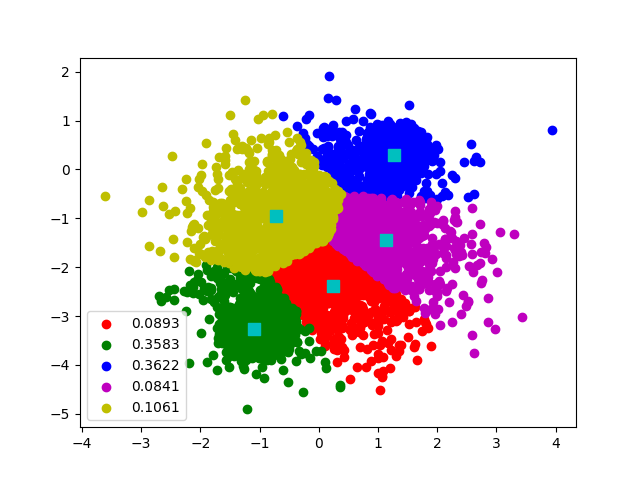
\includegraphics[width=\textwidth]{imgs/kmeans_K_5.png}
        \caption{1.1.3, K = 5}
    \end{subfigure}
\end{figure}

\section{Mixtures of Gaussians}


\section{Discover Latent Dimensions}



\end{document}

